%%%%%%%%%%%%%%%%%%%%%%%%%%%%%%%%%%%%%%%%%%%%%%%%%%%%%%%%%%%%%%%%%%%%%%%%%%%%%%%%%%
\begin{frame}[fragile]\frametitle{}
\begin{center}
{\Large Neo4j}
\end{center}
\end{frame}


%%%%%%%%%%%%%%%%%%%%%%%%%%%%%%%%%%%%%%%%%%%%%%%%%%%%%%%%%%%%%%%%%%%%%%%%%%%%%%%%%%
\begin{frame}\frametitle{Introduction}

\begin{itemize}
\item Open Source
\item Implemented in Java and Scala
\item Cypher : mature and rivals SQL
\item ACID (Atomic, Consistent, Isolated, Durable) compliant
\item Embedded Server
\item REST API
\end{itemize}


\begin{center}
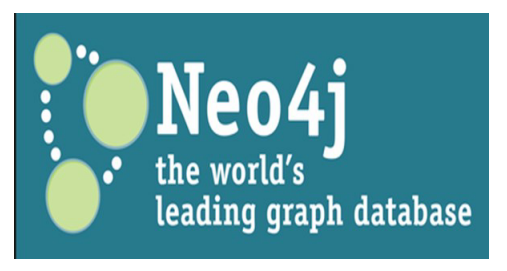
\includegraphics[width=0.2\linewidth,keepaspectratio]{neo4j32}
\end{center}	

{\tiny (Ref: CIS 6930 - Advanced Databases - Neo4j )}
\end{frame}


%%%%%%%%%%%%%%%%%%%%%%%%%%%%%%%%%%%%%%%%%%%%%%%%%%%%%%%%%%%
\begin{frame}[fragile]\frametitle{Neo4j}

\begin{center}
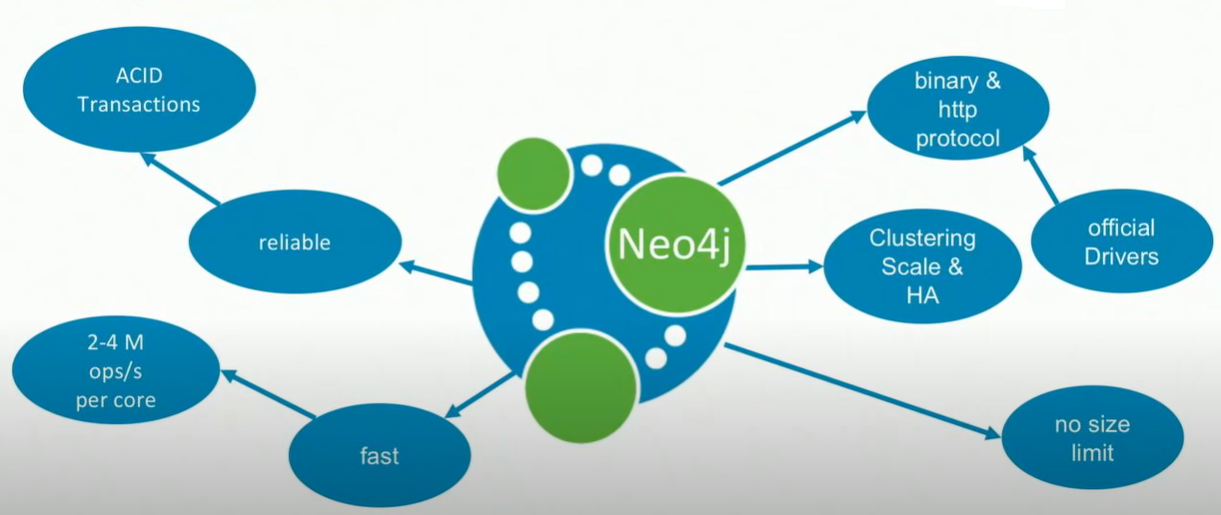
\includegraphics[width=\linewidth,keepaspectratio]{neo4j14}
\end{center}	  

{\tiny (Ref: Introduction to Neo4j and Graph Databases
 - M David Allen)}

\end{frame}

%%%%%%%%%%%%%%%%%%%%%%%%%%%%%%%%%%%%%%%%%%%%%%%%%%%%%%%%%%%%%%%%%%%%%%%%%%%%%%%%%%
\begin{frame}\frametitle{Neo4j features}

\begin{itemize}
\item Capacity: Nodes/Relationships/Labels (all in Billions)
\item High data integrity
\item Native graph processing
\item High scalability
\item Data browser
\end{itemize}

{\tiny (Ref: CIS 6930 - Advanced Databases - Neo4j )}
\end{frame}


%%%%%%%%%%%%%%%%%%%%%%%%%%%%%%%%%%%%%%%%%%%%%%%%%%%%%%%%%%%%%%%%%%%%%%%%%%%%%%%%%%
\begin{frame}\frametitle{Good For}

\begin{itemize}
\item Highly connected data (social networks)
\item Recommendations (e-commerce)
\item Path Finding (how do I know you?)
\item A* (Least Cost path)
\item  Data First Schema (bottom-up, but you still need to design)
\end{itemize}

{\tiny (Ref: CIntroduction to Graph Databases - Max De Marzi )}
\end{frame}

%%%%%%%%%%%%%%%%%%%%%%%%%%%%%%%%%%%%%%%%%%%%%%%%%%%%%%%%%%%%%%%%%%%%%%%%%%%%%%%%%%
\begin{frame}\frametitle{Property Graph}

\begin{center}
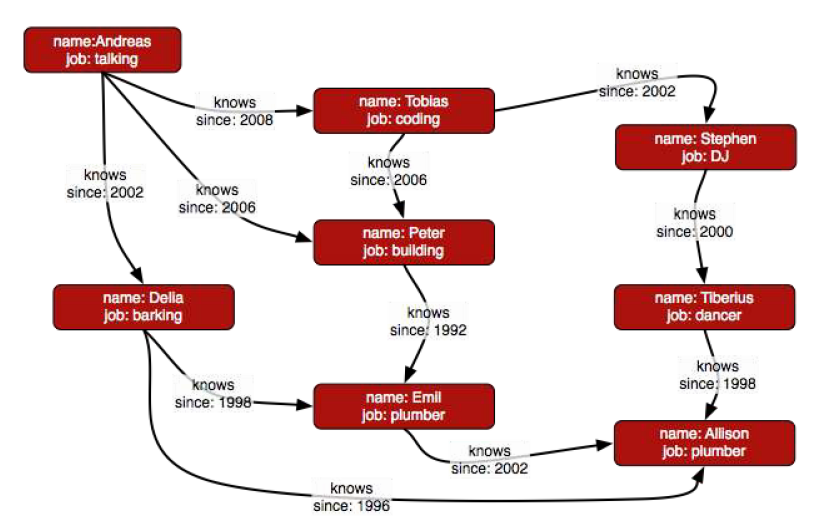
\includegraphics[width=\linewidth,keepaspectratio]{neo4j46}
\end{center}	

{\tiny (Ref: Introduction to Graph Databases - Max De Marzi )}
\end{frame}

%%%%%%%%%%%%%%%%%%%%%%%%%%%%%%%%%%%%%%%%%%%%%%%%%%%%%%%%%%%%%%%%%%%%%%%%%%%%%%%%%%
\begin{frame}\frametitle{Property Graph}

\begin{center}
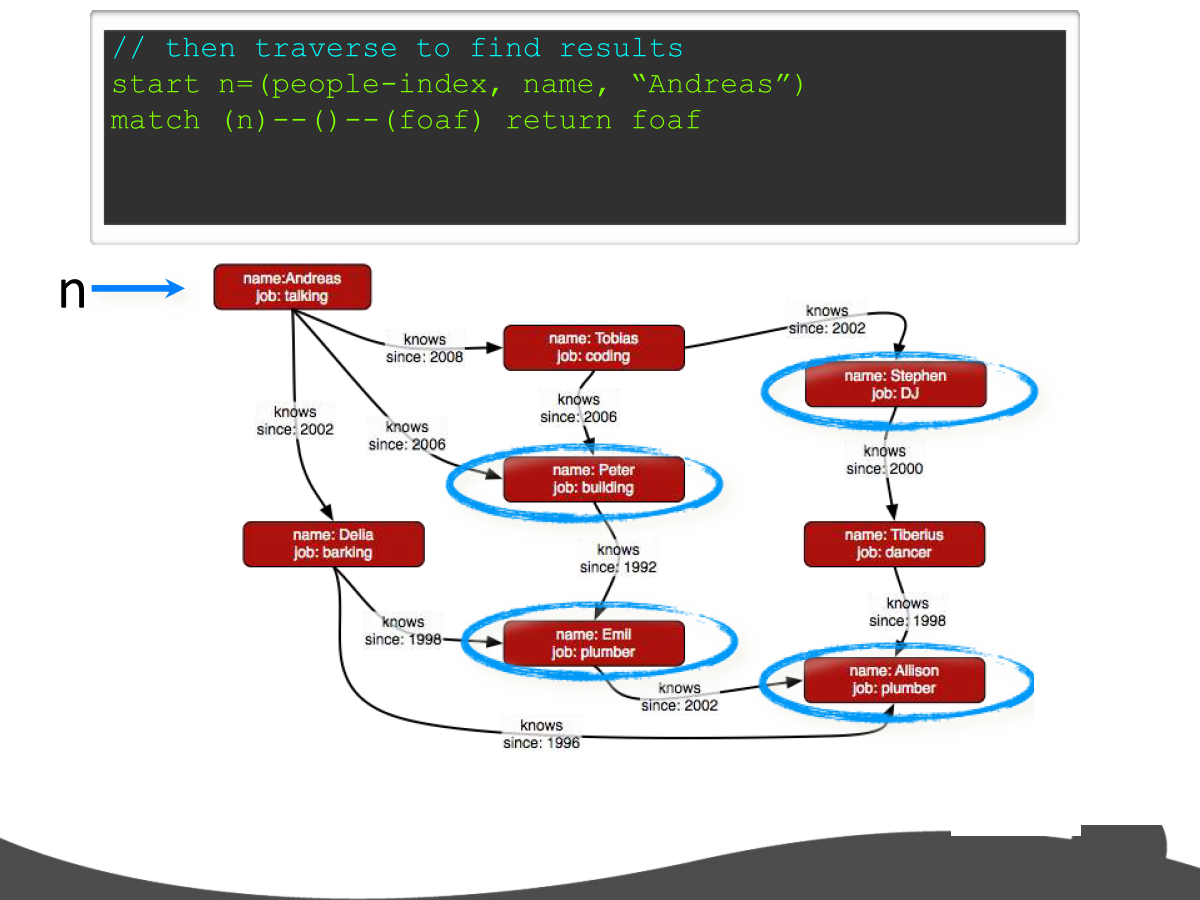
\includegraphics[width=\linewidth,keepaspectratio]{neo4j47}
\end{center}	

{\tiny (Ref: Introduction to Graph Databases - Max De Marzi )}
\end{frame}

%%%%%%%%%%%%%%%%%%%%%%%%%%%%%%%%%%%%%%%%%%%%%%%%%%%%%%%%%%%%%%%%%%%%%%%%%%%%%%%%%%
\begin{frame}\frametitle{Cypher}

Pattern Matching Query Language (like SQL for graphs)

\begin{center}
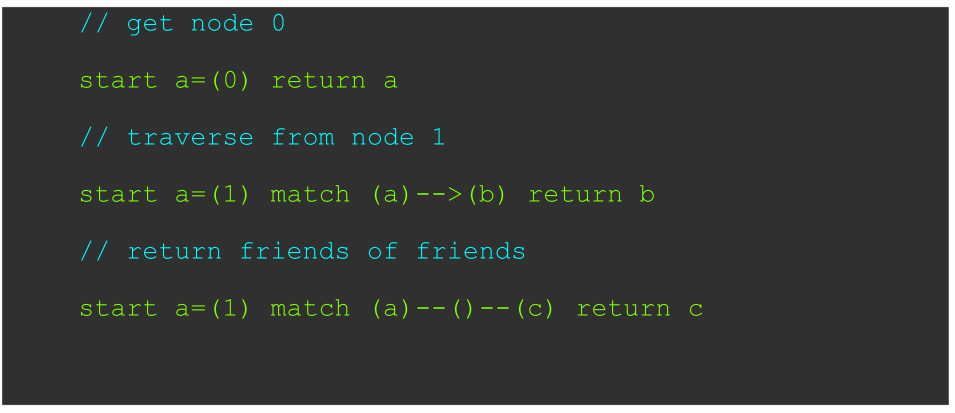
\includegraphics[width=\linewidth,keepaspectratio]{neo4j48}
\end{center}	

{\tiny (Ref: Introduction to Graph Databases - Max De Marzi )}
\end{frame}

%%%%%%%%%%%%%%%%%%%%%%%%%%%%%%%%%%%%%%%%%%%%%%%%%%%%%%%%%%%%%%%%%%%%%%%%%%%%%%%%%%
\begin{frame}\frametitle{Gremlin}

A Graph Scripting DSL (groovy-based)

\begin{center}
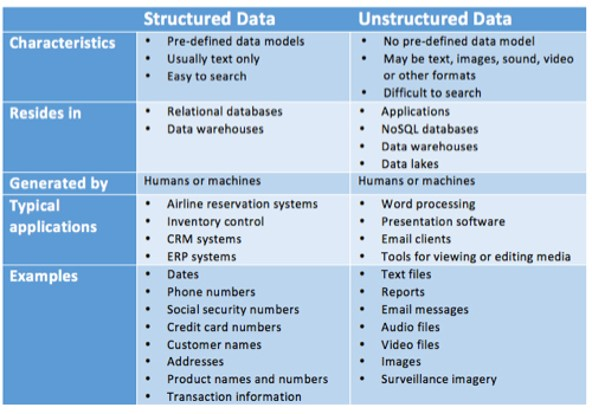
\includegraphics[width=\linewidth,keepaspectratio]{neo4j49}
\end{center}	

{\tiny (Ref: Introduction to Graph Databases - Max De Marzi )}
\end{frame}

%%%%%%%%%%%%%%%%%%%%%%%%%%%%%%%%%%%%%%%%%%%%%%%%%%%%%%%%%%%%%%%%%%%%%%%%%%%%%%%%%%
\begin{frame}\frametitle{If you’ve ever}

\begin{itemize}
\item Joined more than 7 tables together
\item  Modeled a graph in a table
\item  Written a recursive CTE
\item Tried to write some crazy stored procedure with multiple recursive self and inner joins
\end{itemize}

{\bf You should use Neo4j}

{\tiny (Ref: Introduction to Graph Databases - Max De Marzi )}
\end{frame}


%%%%%%%%%%%%%%%%%%%%%%%%%%%%%%%%%%%%%%%%%%%%%%%%%%%%%%%%%%%
\begin{frame}[fragile]\frametitle{Windows Installation}

\begin{itemize}
\item Have Open JDK 11 ready, if not, go to https://learn.microsoft.com/en-us/java/openjdk/download (178 MB)
\item https://neo4j.com/download-center/\#community (4.4.11 129 MB)
\item Place the extracted files in a permanent home on your server, for example \lstinline|D:\neo4j\|. The top level directory is referred to as NEO4J\_HOME.
\item To run Neo4j as a console application, use: \lstinline|<NEO4J_HOME>\bin\neo4j console|

\begin{lstlisting}
C:\neo4j\bin>neo4j.bat console
Directories in use:
home:         C:\neo4j
:
Starting Neo4j.
\end{lstlisting}

\item Visit http://localhost:7474 in your web browser.
\item Default login is username 'neo4j' and password 'neo4j' Change password. Got conncted to `neo4j://127.0.0.1:7687`
\end{itemize}

(Note: Btw, free, no-download sandbox option is available at sandbox.neo4j.com)
\end{frame}

%%%%%%%%%%%%%%%%%%%%%%%%%%%%%%%%%%%%%%%%%%%%%%%%%%%%%%%%%%%%%%%%%%%%%%%%%%%%%%%%%%
\begin{frame}\frametitle{Neo4j Driver API}


\begin{itemize}
\item  Bolt protocol
\item   Currently supports .NET, Java, JavaScript and Python
\item   Uniformity across languages
\end{itemize}


{\tiny (Ref: CIS 6930 - Advanced Databases - Neo4j )}
\end{frame}

%%%%%%%%%%%%%%%%%%%%%%%%%%%%%%%%%%%%%%%%%%%%%%%%%%%%%%%%%%%%%%%%%%%%%%%%%%%%%%%%%%
\begin{frame}\frametitle{Neo4j Browser}


\begin{itemize}
\item   Developer focused
\item    Export results
\item   Visualization
\end{itemize}

\begin{center}
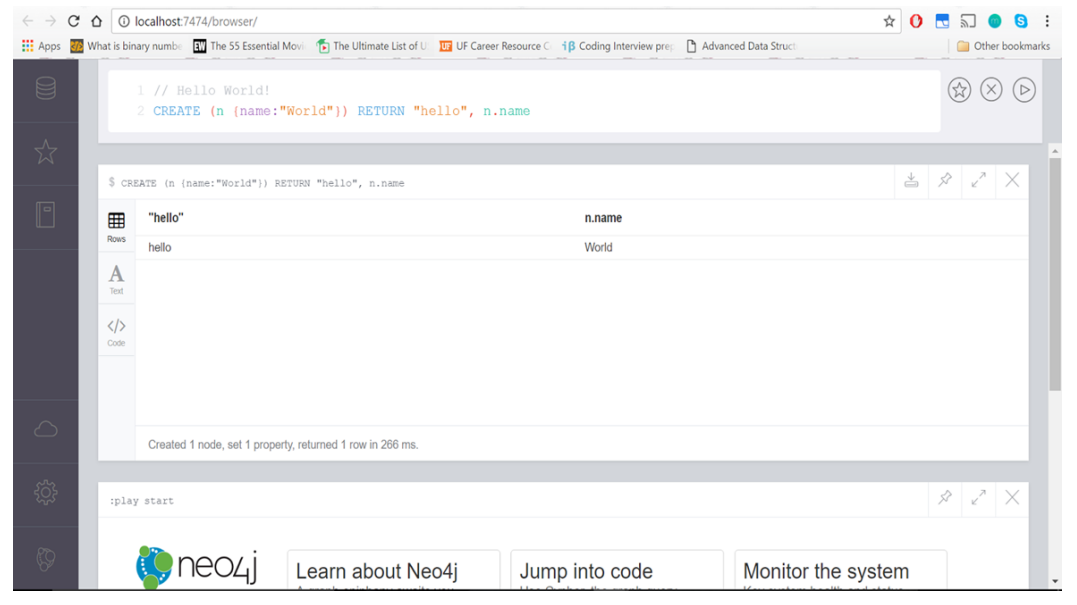
\includegraphics[width=\linewidth,keepaspectratio]{neo4j40}
\end{center}	 

{\tiny (Ref: CIS 6930 - Advanced Databases - Neo4j )}
\end{frame}



%%%%%%%%%%%%%%%%%%%%%%%%%%%%%%%%%%%%%%%%%%%%%%%%%%%%%%%%%%%
\begin{frame}[fragile]\frametitle{Console}

\begin{center}
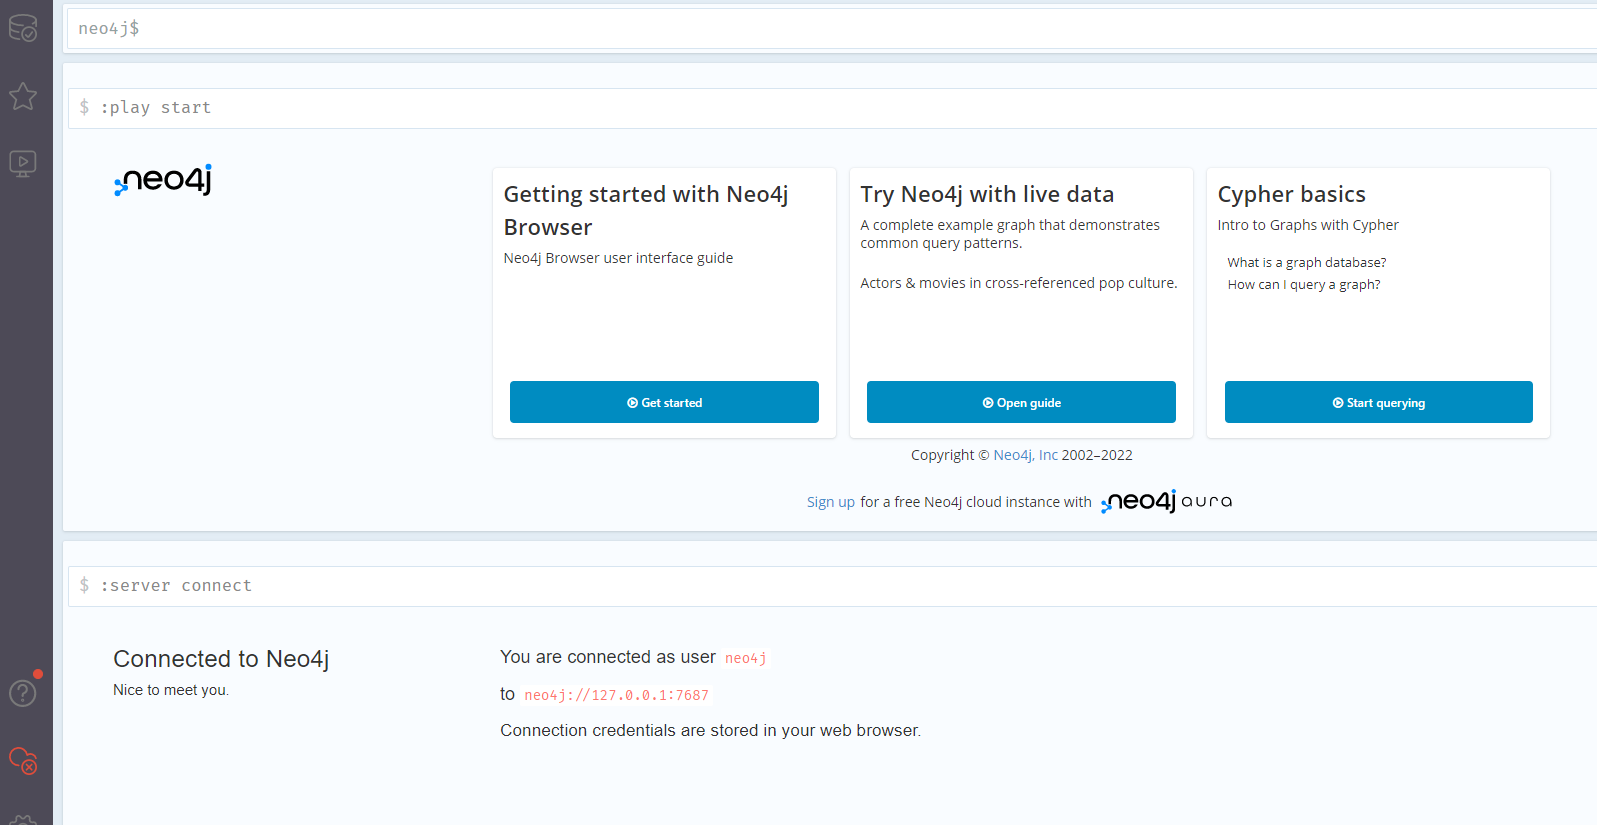
\includegraphics[width=\linewidth,keepaspectratio]{neo4j1}
\end{center}	  


\end{frame}

%%%%%%%%%%%%%%%%%%%%%%%%%%%%%%%%%%%%%%%%%%%%%%%%%%%%%%%%%%%
\begin{frame}[fragile]\frametitle{Interaction}

Type commands in top command window

\begin{itemize}
\item \lstinline|MATCH(n) RETURN n| Return nodes (type none). As there is nothing, nothing gets returned. So create something.
\item \lstinline|CREATE(n)| will create one empty node.
\item \lstinline|MATCH(n) RETURN n| will now return 1 node and show it. $n$ is the reference(s) or the object handle(s), which is returned.
\end{itemize}

\begin{center}
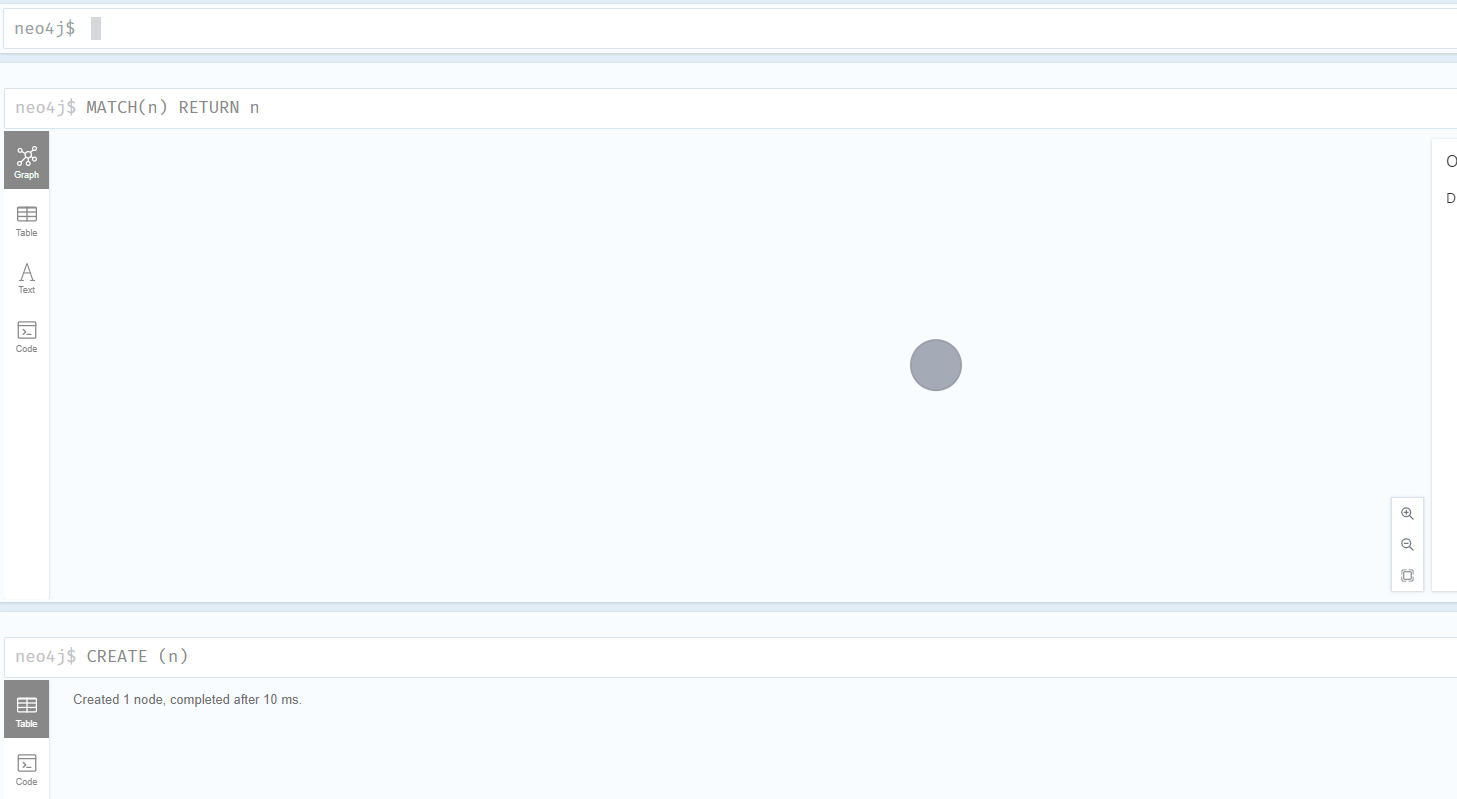
\includegraphics[width=0.8\linewidth,keepaspectratio]{neo4j2}
\end{center}

\end{frame}


%%%%%%%%%%%%%%%%%%%%%%%%%%%%%%%%%%%%%%%%%%%%%%%%%%%%%%%%%%%
\begin{frame}[fragile]\frametitle{Examples}

\begin{itemize}
\item \lstinline|CREATE(n:PERSON)| create a node (type PERSON). Type is actually the label of the node.
\item \lstinline|MATCH(n) DELETE(n)| will delete all the nodes. n, the object handled, returned by MATCH, is getting deleted in the delete function where n is argument. 
\item \lstinline|CREATE(n:PERSON{name:'chris', favoritecolor:'blue'})| create a node (type PERSON) along with some properties. SImilariy, can create different nodes of different type.
\item \lstinline|MATCH(n:PERSON) RETURN n|to selectively return only PERSONs.
\item \lstinline|MATCH(n) RETURN n LIMIT 4| to return only 4 nodes
\item Two create relationship find 2 nodes using \lstinline|MATCH| and \lstinline|WHERE| to restrict, then create relationship 'studied\_at'

\begin{lstlisting}
MATCH (s:School), (p:Person)
WHERE s.name = 'LSU' and p.name = 'jenny'
CREATE (p)-[stu:STUDIED_AT]->(s)
\end{lstlisting}


\end{itemize}

\end{frame}


%%%%%%%%%%%%%%%%%%%%%%%%%%%%%%%%%%%%%%%%%%%%%%%%%%%%%%%%%%%
\begin{frame}[fragile]\frametitle{Examples}


\begin{center}
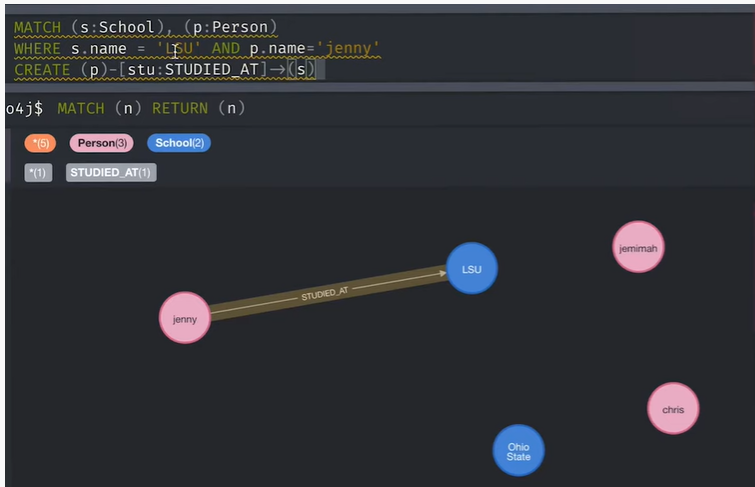
\includegraphics[width=0.9\linewidth,keepaspectratio]{neo4j3}
\end{center}	

{\tiny (Ref: An introduction to neo4j (graph database tutorial for beginners) - Chris Hay)}

\end{frame}

%%%%%%%%%%%%%%%%%%%%%%%%%%%%%%%%%%%%%%%%%%%%%%%%%%%%%%%%%%%
\begin{frame}[fragile]\frametitle{Comparison}
Find all reports and how many people they manage upto 3 levels down.

\begin{center}
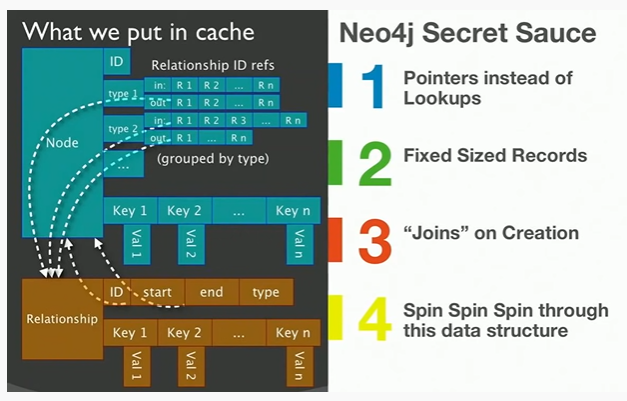
\includegraphics[width=\linewidth,keepaspectratio]{neo4j20}
\end{center}	    

{\tiny (Ref: Introduction to Neo4j and Graph Databases
 - M David Allen)}

\end{frame}

%%%%%%%%%%%%%%%%%%%%%%%%%%%%%%%%%%%%%%%%%%%%%%%%%%%%%%%%%%%
\begin{frame}[fragile]\frametitle{Choice}
When to choose Neo4j over Relational databases? Sub-second response \ldots


\begin{center}
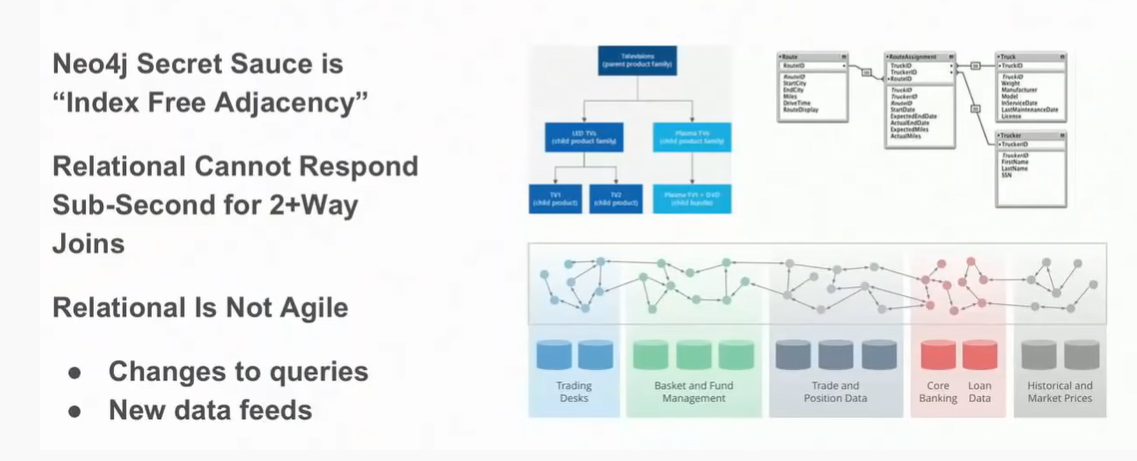
\includegraphics[width=\linewidth,keepaspectratio]{neo4j21}
\end{center}	    

{\tiny (Ref: Introduction to Neo4j and Graph Databases
 - M David Allen)}

\end{frame}

%%%%%%%%%%%%%%%%%%%%%%%%%%%%%%%%%%%%%%%%%%%%%%%%%%%%%%%%%%%%%%%%%%%%%%%%%%%%%%%%%%
\begin{frame}\frametitle{Neo4j Drawbacks}


\begin{itemize}
\item  Scalability
\item   Complex Domains
\item   Complex types
\item   Deleted Records
\end{itemize}

 

{\tiny (Ref: CIS 6930 - Advanced Databases - Neo4j )}
\end{frame}

%%%%%%%%%%%%%%%%%%%%%%%%%%%%%%%%%%%%%%%%%%%%%%%%%%%%%%%%%%%%%%%%%%%%%%%%%%%%%%%%%%
\begin{frame}[fragile]\frametitle{}
\begin{center}
{\Large Architecture}
\end{center}
\end{frame}

%%%%%%%%%%%%%%%%%%%%%%%%%%%%%%%%%%%%%%%%%%%%%%%%%%%%%%%%%%%%%%%%%%%%%%%%%%%%%%%%%%
\begin{frame}\frametitle{Native Graph Processing}



\begin{itemize}
\item Index-free adjacency
\item Each node maintains direct references to its adjacent nodes
\item Efficient query time
\end{itemize}

{\tiny (Ref: CIS 6930 - Advanced Databases - Neo4j )}
\end{frame}

%%%%%%%%%%%%%%%%%%%%%%%%%%%%%%%%%%%%%%%%%%%%%%%%%%%%%%%%%%%%%%%%%%%%%%%%%%%%%%%%%%
\begin{frame}\frametitle{Native Graph Storage}

\begin{center}
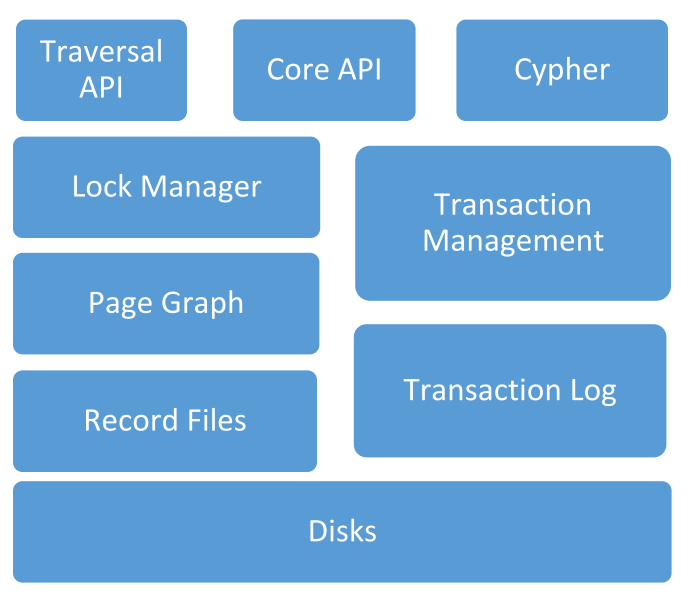
\includegraphics[width=0.5\linewidth,keepaspectratio]{neo4j37}
\end{center}	  


{\tiny (Ref: CIS 6930 - Advanced Databases - Neo4j )}
\end{frame}

%%%%%%%%%%%%%%%%%%%%%%%%%%%%%%%%%%%%%%%%%%%%%%%%%%%%%%%%%%%%%%%%%%%%%%%%%%%%%%%%%%
\begin{frame}\frametitle{Native Graph Storage}

\begin{center}
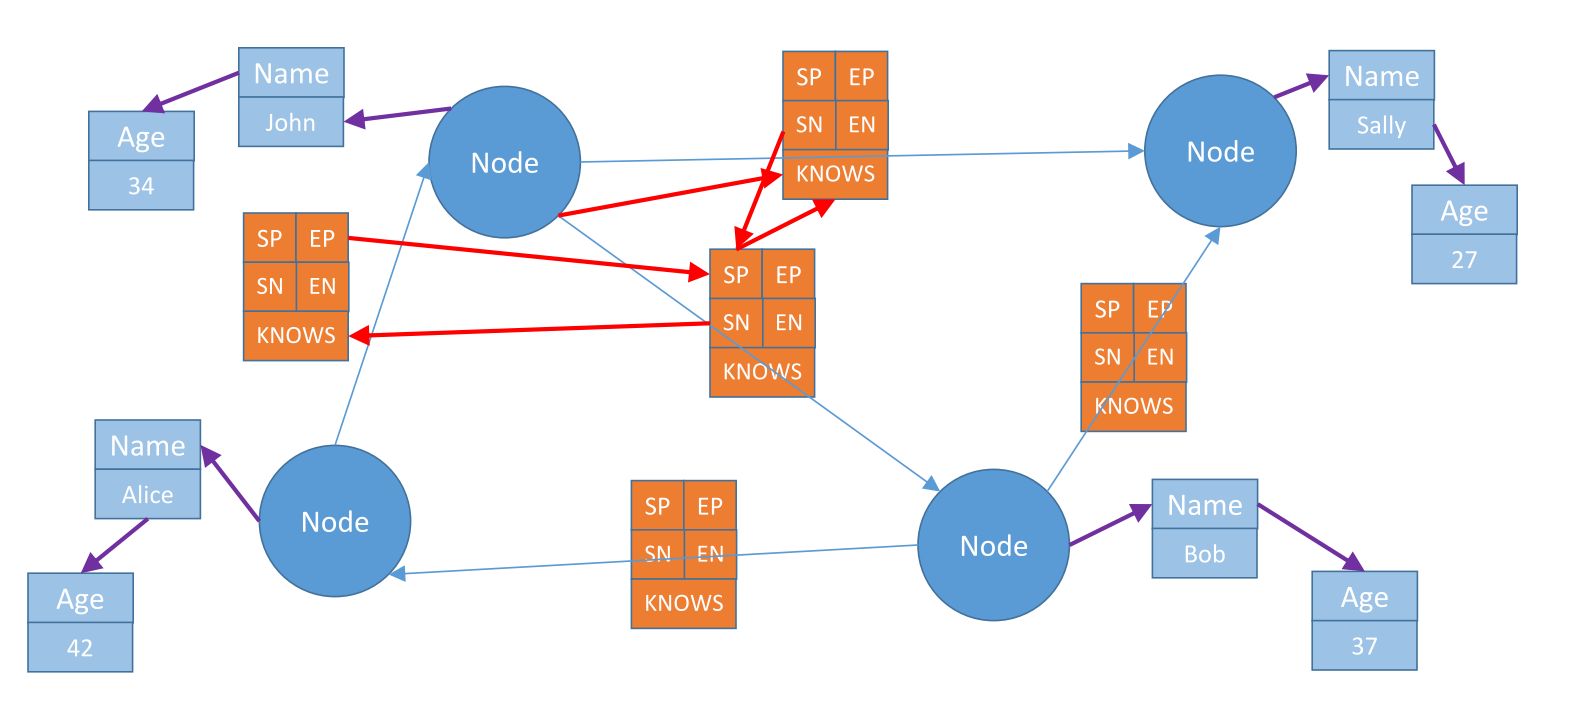
\includegraphics[width=\linewidth,keepaspectratio]{neo4j38}
\end{center}	  


{\tiny (Ref: CIS 6930 - Advanced Databases - Neo4j )}
\end{frame}

%%%%%%%%%%%%%%%%%%%%%%%%%%%%%%%%%%%%%%%%%%%%%%%%%%%%%%%%%%%%%%%%%%%%%%%%%%%%%%%%%%
\begin{frame}\frametitle{Cypher Query Language}

\begin{itemize}
\item Neo4j’s open graph query language
\item Uses patterns to describe graph data
\item Familiar SQL-like clauses
\item Describe what to find, not how to find it
\end{itemize}

{\tiny (Ref: CIS 6930 - Advanced Databases - Neo4j )}
\end{frame}
